\documentclass[12pt, oneside, openany]{book}

%----------------------------------------------
% Encoding and Typography Enhancements
%----------------------------------------------
\usepackage[T1]{fontenc}            % Enhanced font encoding
\usepackage[utf8]{inputenc}         % Direct Unicode input
\usepackage{microtype}              % Fine-tune character spacing for better typography

%----------------------------------------------
% Primary and Mathematical Fonts
%----------------------------------------------
\usepackage{charter}                % Charter: legible serif for body text
\usepackage{mathpazo}               % Palatino-like math fonts
\usepackage{bm}                     % Bold math symbols

%----------------------------------------------
% Monospaced Font for Code Listings
%----------------------------------------------
\usepackage[scaled=.95]{inconsolata} % Inconsolata for code

%----------------------------------------------
% Page Layout and Spacing
%----------------------------------------------
\usepackage[a4paper, margin=1in]{geometry} % 1" margins on A4
\usepackage{setspace}              % Line-spacing control
\setstretch{1.3}                   % 1.3× line spacing

%----------------------------------------------
% Headers and Footers
%----------------------------------------------
\usepackage{fancyhdr}              % Fancy header/footer
\pagestyle{fancy}
\fancyhf{}
\fancyhead[L]{\nouppercase{\leftmark}} % Chapter title on left
\fancyhead[R]{\thepage}               % Page number on right
\fancypagestyle{plain}{               % Plain pages (e.g., chapter starts)
	\fancyhf{}
	\fancyfoot[C]{\thepage}
}

%----------------------------------------------
% Hyperlinks and PDF Metadata
%----------------------------------------------
\usepackage{hyperref}
\hypersetup{
	colorlinks    = true,
	linkcolor     = black,    % Internal links in black (print-friendly)
	citecolor     = blue,     % Citation links in blue
	urlcolor      = cyan,     % URLs in cyan
	pdfauthor     = {Mahdi},
	pdftitle      = {Arliz},
	pdfsubject    = {Programming, Arrays, and Data Structures},
	pdfkeywords   = {Arrays, Data Structures, Programming, History of Computing}
}

%----------------------------------------------
% Graphics and Diagrams
%----------------------------------------------
\usepackage{graphicx}             % Include images
\usepackage{caption}              % Customize captions
\usepackage{subcaption}           % Sub-figures support
\usepackage{xcolor}               % Color definitions
\usepackage{tikz}                 % Vector graphics & diagrams
\usetikzlibrary{positioning, shapes.geometric, arrows, calc}

%----------------------------------------------
% Tables and Arrays
%----------------------------------------------
\usepackage{array}                % Extended tabular features

%----------------------------------------------
% Section and Title Formatting
%----------------------------------------------
\usepackage{titlesec}             % Control title styles
\titleformat{\chapter}[display]
{\normalfont\huge\bfseries}{\chaptername\ \thechapter}{20pt}{\Huge}
\titleformat{\section}
{\Large\bfseries}{\thesection}{1em}{}
\titleformat{\subsection}
{\large\bfseries}{\thesubsection}{1em}{}

%----------------------------------------------
% Code Listings and Pseudocode
%----------------------------------------------
\usepackage{listings}             % Source code highlighting
\lstset{
	basicstyle      = \ttfamily\small,
	frame           = single,
	breaklines      = true,
	numbers         = left,
	numberstyle     = \tiny\color{gray},
	keywordstyle    = \color{myblue}\bfseries,
	commentstyle    = \color{olive},
	stringstyle     = \color{orange},
	backgroundcolor = \color{lightgray!20},
	captionpos      = b,
	escapeinside    = {(*@}{@*)},
	morekeywords    = {array, structure, algorithm, complexity}
}

\usepackage{algorithm}             % Algorithm floats
\usepackage{algpseudocode}         % Pseudocode environment

%----------------------------------------------
% Color Definitions
%----------------------------------------------
\definecolor{myblue}{RGB}{0, 102, 204}     % Custom blue for code
\definecolor{lightgray}{RGB}{240, 240, 240} % Light gray background

%----------------------------------------------
% Special Boxes and Environments
%----------------------------------------------
\usepackage{tcolorbox}
\tcbuselibrary{most}

\newtcolorbox{notebox}[1][]{
	colback   = blue!5!white,
	colframe  = blue!75!black,
	title     = Note,
	#1
}
\newtcolorbox{tipbox}[1][]{
	colback   = green!5!white,
	colframe  = green!75!black,
	title     = Tip,
	#1
}
\newtcolorbox{warningbox}[1][]{
	colback   = red!5!white,
	colframe  = red!75!black,
	title     = Important,
	#1
}

%----------------------------------------------
% Bibliography and Citations
%----------------------------------------------
\usepackage[backend=biber,style=apa]{biblatex}
\addbibresource{references.bib}

%----------------------------------------------
% Table of Contents, Bibliography, Index
%----------------------------------------------
\usepackage{tocbibind}            % Include TOC adds
\usepackage{imakeidx}             % Index creation
\makeindex

%----------------------------------------------
% Multiple Columns (e.g., Glossary)
%----------------------------------------------
\usepackage{multicol}

%----------------------------------------------
% PDF Inclusion (e.g., for front matter pages)
%----------------------------------------------
\usepackage{pdfpages}
\begin{document}
	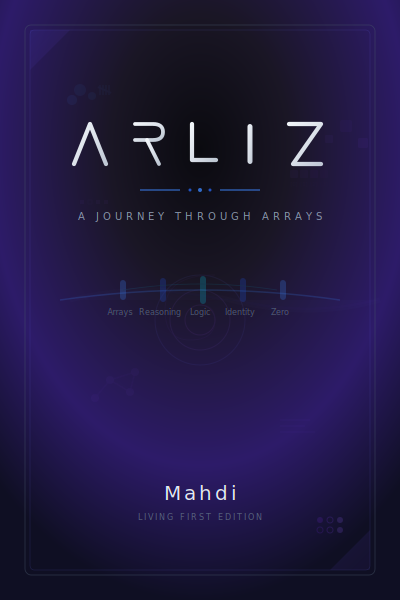
\includepdf[pages=-, pagecommand={\thispagestyle{empty}}, width=\paperwidth, height=\paperheight]{logo.pdf}
	
	\frontmatter
	% Title Page (Front Matter)

\begin{titlepage}
	\begin{center}
		\vspace*{2cm}

		{\Huge\bfseries In Praise of Arliz}\\[2em]
		
		{\Large\scshape Mahdi}\\[0.5em]
		
		\begin{minipage}{1\textwidth}
			\centering
			This book evolves. Every insight gained—whether a circuit, a structure,\\
				or a simple idea—is absorbed and integrated. 
		\end{minipage}
		
		\vfill
		
	{\large \textsc{First Edition}}\\[0.5em]
	{\large \today}
	
	\vspace*{1cm}
	{\small
		\textcopyright\ 2025 Mahdi “Genix”  
		\par
		Released under the MIT License  
	}
	\end{center}
\end{titlepage}

%----------------------------------------------
% Dedication
%----------------------------------------------
\thispagestyle{empty}
\vspace*{6cm}
\begin{center}
	\emph{
		To those who build from first principles.\\
		To the silent thinkers who design before they speak.\\
		To the ones who see in systems—\\
		not just machines, but metaphors.\\
		This is for you.}
\end{center}

\pagestyle{empty}
	\chapter*{Preface}
	\thispagestyle{empty}

	%\maketitle
	Every book has its own story, and this book is no exception. If I were to summarize the process of creating this book in one word, that word would be “improvised.” Yet the truth is that Arliz is the result of pure, persistent curiosity that has grown in my mind for years. What you are reading now could be called a technical book, a collection of personal notes, or even a journal of unanswered questions and curiosities. But I—officially—call it a \emph{book}, because it is written not only for others but for myself, as a record of my learning journey and an effort to understand more precisely the concepts that once seemed obscure and, at times, frustrating.\\
	The story of Arliz began with a simple feeling: \textbf{curiosity}.  
	Curiosity about what an array truly is. Perhaps for many this question seems trivial, but for me this word—encountered again and again in algorithm and data structure discussions—always raised a persistent question.\\
	Every time I saw terms like \texttt{array}, \texttt{stack}, \texttt{queue}, \texttt{linked list}, \texttt{hash table}, or \texttt{heap}, I not only felt confused but sensed that something fundamental was missing. It was as if a key piece of the puzzle had been left out. The first brief, straightforward explanations I found in various sources never sufficed; they assumed you already knew exactly what an array is and why you should use it. But I was looking for the \emph{roots}. I wanted to understand from zero what an array means, how it was born, and what hidden capacities it holds.\\
	That realization led me to decide:  
	\emph{If I truly want to understand, I must start from zero.}\\	
	There is no deeper story behind the name “Arliz.” There is no hidden philosophy or special inspiration—just a random choice. I simply declared:  
	\emph{This book is called Arliz.}  
	You may pronounce it "Ar-liz," "Array-Liz," or any way you like. I personally say "ar-liz." That is all—simple and arbitrary.\\	
	But Arliz is not merely a technical book on data structures. In fact, \textbf{Arliz grows alongside me}. \\
	Whenever I learn something I deem worth writing, I add it to this book. Whenever I feel a section could be explained better or more precisely, I revise it. Whenever a new idea strikes me—an algorithm, an exercise, or even a simple diagram to clarify a structure—I incorporate it into Arliz.\\
	This means Arliz is a living project. As long as I keep learning, Arliz will remain alive.\\	
	The structure of this book has evolved around a simple belief: true understanding begins with context. That’s why Arliz doesn’t start with code or syntax, but with the origins of computation itself. We begin with the earliest tools and ideas—counting stones, the abacus, mechanical gears, and early notions of logic—long before transistors or binary digits came into play. From there, we follow the evolution of computing: from ancient methods of calculation to vacuum tubes and silicon chips, from Babbage’s Analytical Engine to the modern microprocessor. Along this journey, we discover that concepts like arrays aren’t recent inventions—they are the culmination of centuries of thought about how to structure, store, and process information.\\
	In writing this book, I have always tried to follow three principles:
	
	\begin{itemize}
		\item \textbf{Simplicity of Expression:} I strive to present concepts in the simplest form possible, so they are accessible to beginners and not superficial or tedious for experienced readers.
		\item \textbf{Concept Visualization:} I use diagrams, figures, and visual examples to explain ideas that are hard to imagine, because I believe visual understanding has great staying power.
		\item \textbf{Clear Code and Pseudocode:} Nearly every topic is accompanied by code that can be easily translated into major languages like C\texttt{++}, Java, or C\#, aiming for both clarity and practicality.
	\end{itemize}
	
	An important note: many of the algorithms in Arliz are implemented by myself. I did not copy them from elsewhere, nor are they necessarily the most optimized versions. My goal has been to understand and build them from scratch rather than memorize ready-made solutions. Therefore, some may run slower than standard implementations—or sometimes even faster. For me, the process of understanding and constructing has been more important than simply reaching the fastest result.\\	
	Finally, let me tell you a bit about myself:  
	I am \textbf{Mehdi}. If you prefer, you can call me by my alias: \emph{Genix}. I am a student of Computer Engineering (at least at the time of writing this). I grew up with computers—from simple games to typing commands in the terminal—and I have always wondered what lies behind this screen of black and green text. There is not much you need to know about me, just that I am someone who works with computers, sometimes gives them commands, and sometimes learns from them.\\	
	I hope this book will be useful for understanding concepts, beginning your learning journey, or diving deeper into data structures. \\	
	Arliz is freely available. You can access the PDF, LaTeX source, and related code at:  
	\begin{center}
		\url{https://github.com/m-mdy-m/Arliz}
	\end{center}
	In each chapter, I have included exercises and projects to aid your understanding. Please do not move on until you have completed these exercises, because true learning happens only by solving problems.\\	
	I hope this book serves you well—whether for starting out, reviewing, or simply satisfying your curiosity. And if you learn something, find an error, or have a suggestion, please let me know. As I said:
	\emph{This book grows with me.}
	
	% Acknowledgments
	\pagestyle{empty}
	\chapter*{Acknowledgments}
		\thispagestyle{empty}
		I would like to express my gratitude to everyone who supported me during the creation of this book. Special thanks to the open-source community for their invaluable resources and to all those who reviewed early drafts and provided feedback.
		
		%\maketitle

	\tableofcontents
	\renewcommand{\arraystretch}{1.5} % Adjust row height for better readability
% Main Content
\mainmatter

\part{The Birth of Computing: From Mechanical to Electronic}

\section*{Introduction}

Long before a single line of code was ever written—long before electricity, transistors, or even the concept of modern logic circuits—humans felt an innate drive to calculate, record, and model the world around them. Computing is not a recent invention. It is one of humanity’s oldest intellectual pursuits, rooted in necessity and evolved through creativity. Before we dive into complex abstractions like arrays or data structures, we must ask a deeper, almost philosophical question: \textbf{What does it mean to compute?}\\
This part of the book invites you on a journey—not just through the machinery and breakthroughs that brought us the modern computer, but through the evolution of human thought about numbers, representation, and control. Arrays, as we will later explore in depth, are not merely structures to store data. They are reflections of how we’ve ordered information for thousands of years. Their logic is built upon ancient insights—on sets, sequences, and patterns—and they embody the fundamental human need to represent, repeat, and manipulate structured information.\\
Our journey begins in ancient times, long before Christ, with devices like the abacus, first appearing over 2,500 years ago in Mesopotamia and later refined by Chinese, Roman, and Japanese cultures. The abacus was not just a calculator—it was an embodiment of the concepts of \textbf{state}, \textbf{position}, and \textbf{transformation}, principles that continue to underpin all modern computation. It allowed people to model quantities, track multiple values in parallel (an early echo of array indexing), and perform operations based on positional representation.\\
From these early tools, we progress into the classical mathematical age, where the Greeks formalized logic, and concepts like \textbf{sets} and \textbf{ordered lists} began to take philosophical shape. While not arrays in the modern sense, these ideas laid the intellectual groundwork for thinking about groups of data—grouped, related, or sequential—that could be acted upon as a whole. The set, in particular, became a foundational concept in mathematics and later in programming: an abstract container for elements that obey rules and enable operations. The leap from abstract sets to concrete arrays reflects one of the key transitions in computational history—from idea to implementation.\\
In the 17th century, visionaries like Blaise Pascal and Gottfried Wilhelm Leibniz attempted to automate arithmetic with mechanical devices. These weren’t just clever tools—they were the first signs of a dream to make thinking itself mechanical. Charles Babbage expanded this dream with his Analytical Engine in the 19th century, envisioning a machine that could be programmed and reprogrammed—a concept that wouldn’t become reality until a century later. Ada Lovelace, who worked with Babbage, went even further. She grasped that machines could go beyond numbers: they could process symbolic logic, follow instructions, and even imitate aspects of reasoning. She anticipated the algorithm as a mental construct, not just a set of steps.\\
As we move forward into the 20th century, the invention of electromechanical and electronic machines—using relays, vacuum tubes, and later transistors—marked a revolution. No longer limited by gears and levers, computers became faster, more reliable, and more abstract. The idea of a \textbf{stored program} emerged, allowing machines to modify their behavior dynamically. This wasn’t just a technical innovation—it was a conceptual transformation. Programs became data, and data became active. Arrays, now implemented in memory, could be changed, traversed, and manipulated at runtime—opening the door to software as we know it today.\\
Eventually, we arrive at logic gates, boolean algebra, and the transistor—the atomic units of modern computation. These are more than circuits; they are the physical embodiment of logical thought: conditions, branching, repetition. From gates we build circuits, from circuits microprocessors, and from those, machines that can simulate anything we can formalize.\\
Before concluding this part, we will look closely at how data is represented: binary numbers, encoding schemes, floating-point formats, and character representations. These are not just technical tools; they are perspectives. They define the limits of what a machine can know, express, and manipulate. And finally, we arrive at memory—where arrays live, grow, and function. Memory is not just storage; it is the canvas of computation. It is where change happens and where order emerges.\\
If you are excited to write code, build systems, and jump into implementation, you are free to skip ahead. But if you stay with us for this brief but essential historical and conceptual journey, you will see programming not just as control over a machine, but as part of a much older story: the story of how humans learned to structure thought, encode logic, and make abstract ideas come alive.\\
Let us begin—at the beginning. With sand, stone, wood, and brass. And with minds bold enough to imagine machines that think.

% ==========================================
% CHAPTER 1: PHILOSOPHICAL FOUNDATIONS
% ==========================================

\chapter{What Does It Mean to Compute?}

\section{The Human Urge to Measure and Represent}
\subsection{The Birth of Abstraction: From Reality to Symbol}
\subsection{Quantity, Quality, and the Need for Order}
\subsection{The Cognitive Origins of Structured Thinking}

\section{From Counting Stones to Conceptual Models}
\subsection{Tally Marks and Primitive State}
\subsubsection{The Concept of Discrete Representation}
\subsubsection{Position and Value: Early Insights}
\subsubsection{One-to-One Correspondence}

\subsection{Abstraction and the Birth of Mathematical Thought}
\subsubsection{From Concrete to Abstract Numbers}
\subsubsection{The Emergence of Zero and Infinity}
\subsubsection{Symbolic Manipulation vs. Physical Reality}

\section{Mathematical Roots of Arrays}
\subsection{Sets, Sequences, and Order}
\subsubsection{Euclid's Elements: Systematic Organization}
\subsubsection{The Concept of Mathematical Collections}
\subsubsection{Ordered vs. Unordered Structures}

\subsection{The Notion of Indexing and Mapping}
\subsubsection{Coordinate Systems in Ancient Mathematics}
\subsubsection{Positional Notation Systems}
\subsubsection{Functions and Mappings: Early Abstractions}

\subsection{From Euclid to Euler: Structure in Mathematical Systems}
\subsubsection{Systematic Proofs and Logical Sequences}
\subsubsection{Graph Theory and Relational Structures}
\subsubsection{The Bridge to Modern Data Organization}

% ==========================================
% CHAPTER 2: ANCIENT COMPUTING TOOLS
% ==========================================

\chapter{Ancient Tools of Structured Computation}

\section{The Abacus: Humanity's First Array-Like Structure}
\subsection{Mesopotamian Origins and Clay Tokens}
\subsubsection{Token Systems as Discrete Data Storage}
\subsubsection{Positional Value and Place Representation}
\subsubsection{The Transition from Tokens to Beads}

\subsection{Chinese Suanpan: Parallel Processing in Wood}
\subsubsection{Bi-quinary System Implementation}
\subsubsection{Multi-Column Operations and Carry Logic}
\subsubsection{The Art of Mental-Physical Coordination}

\subsection{Roman and Japanese Variants}
\subsubsection{Soroban: Precision and Efficiency}
\subsubsection{Cultural Adaptations and Regional Optimizations}
\subsubsection{Speed Computing Techniques}

\subsection{Philosophical Implications of the Abacus}
\subsubsection{State, Transformation, and Memory}
\subsubsection{Parallel Computation in Ancient Times}
\subsubsection{The Abacus as a Programming Interface}

\section{Ancient Number Tables: Proto-Arrays in Practice}
\subsection{Babylonian Mathematical Tablets}
\subsubsection{Multiplication Tables in Cuneiform}
\subsubsection{Square and Cube Root Tables}
\subsubsection{Astronomical Computation Tables}
\subsubsection{Two-Dimensional Data Organization}

\subsection{Egyptian Mathematical Papyri}
\subsubsection{Rhind Papyrus: Systematic Problem Solutions}
\subsubsection{Unit Fraction Tables and Decomposition}
\subsubsection{Geometric Progression Tables}
\subsubsection{Tabular Methods for Complex Calculations}

\section{Chinese Rod Numerals and Matrix Operations}
\subsection{The Rod Numeral System}
\subsubsection{Physical Representation of Abstract Numbers}
\subsubsection{Spatial Arrangement and Value}
\subsubsection{Early Binary-Like Concepts}

\subsection{Ancient Matrix Calculations}
\subsubsection{Simultaneous Linear Equations}
\subsubsection{The Nine Chapters on Mathematical Art}
\subsubsection{Gaussian Elimination in Ancient China}
\subsubsection{Matrix as a Computational Tool}

\subsection{Multiplication Matrices and Lookup Tables}
\subsubsection{Pre-computed Result Storage}
\subsubsection{Cross-Reference Systems}
\subsubsection{Error Checking and Verification Methods}

% ==========================================
% CHAPTER 3: MEDIEVAL AND RENAISSANCE
% ==========================================

\chapter{Medieval and Renaissance: Systematization of Knowledge}

\section{Islamic Golden Age Contributions}
\subsection{Al-Khwarizmi and Algorithmic thinking}
\subsubsection{The Word Algorithm and Its Origins}
\subsubsection{Systematic Problem-Solving Procedures}
\subsubsection{Algebra as Structured Manipulation}

\subsection{Mathematical Tables and Astronomical Calculations}
\subsubsection{Zij Tables: Astronomical Arrays}
\subsubsection{Trigonometric Function Tables}
\subsubsection{Precision and Interpolation Techniques}

\section{Renaissance Calculating Tools}
\subsection{Calculating Rods and Napier's Bones}
\subsubsection{John Napier's Logarithmic Innovation}
\subsubsection{Physical Implementation of Multiplication}
\subsubsection{Modular Arithmetic Tools}

\subsection{Mathematical Tables Revolution}
\subsubsection{Printed Logarithm Tables}
\subsubsection{Trigonometric Function Collections}
\subsubsection{Navigation and Scientific Computation}
\subsubsection{Error Propagation and Accuracy}

\section{The Emergence of Systematic Notation}
\subsection{Symbolic Algebra Development}
\subsubsection{François Viète and Symbolic Mathematics}
\subsubsection{The Power of Abstract Representation}
\subsubsection{From Numbers to Variables}

\subsection{Coordinate Systems and Cartesian Innovation}
\subsubsection{René Descartes and Analytical Geometry}
\subsubsection{Two-Dimensional Data Representation}
\subsubsection{Functions as Mappings}

% ==========================================
% CHAPTER 4: MECHANICAL COMPUTATION
% ==========================================

\chapter{Mechanical Computation: The Dream of Automated Thinking}

\section{Early Mechanical Calculators}
\subsection{Blaise Pascal's Pascaline}
\subsubsection{Mechanical Carry Implementation}
\subsubsection{Decimal Wheel Systems}
\subsubsection{The Challenge of Mechanical Precision}

\subsection{Leibniz's Stepped Reckoner}
\subsubsection{Four-Function Arithmetic Machine}
\subsubsection{The Leibniz Wheel Innovation}
\subsubsection{Mechanical Logic and Binary Concepts}

\section{Charles Babbage's Visionary Machines}
\subsection{The Difference Engine}
\subsubsection{Polynomial Calculation Automation}
\subsubsection{Method of Finite Differences}
\subsubsection{Precision Manufacturing Challenges}

\subsection{The Analytical Engine: First Programmable Computer}
\subsubsection{Separation of Processing and Memory}
\subsubsection{The Mill and the Store}
\subsubsection{Punched Card Programming}
\subsubsection{Conditional Branching and Loops}

\section{Ada Lovelace: The First Programmer}
\subsection{Understanding the Analytical Engine}
\subsubsection{Beyond Pure Calculation}
\subsubsection{Symbolic Processing Possibilities}
\subsubsection{The Concept of a Stored Program}

\subsection{Lovelace's Algorithm}
\subsubsection{Bernoulli Numbers Calculation}
\subsubsection{First Computer Program in History}
\subsubsection{Loop Structures and Iteration}

% ==========================================
% CHAPTER 5: ELECTROMECHANICAL ERA
% ==========================================

\chapter{The Electromechanical Revolution}

\section{From Mechanical to Electrical}
\subsection{Telegraph and Early Electrical Logic}
\subsubsection{Boolean Algebra in Physical Form}
\subsubsection{Relay-Based Switching Systems}
\subsubsection{Binary State Representation}

\subsection{Hollerith's Tabulating Machine}
\subsubsection{1890 US Census Automation}
\subsubsection{Punched Card Data Processing}
\subsubsection{Statistical Analysis Machines}

\section{Early 20th Century Computing Machines}
\subsection{Konrad Zuse's Z-Series}
\subsubsection{Z1: Mechanical Binary Computer}
\subsubsection{Z3: First Working Programmable Computer}
\subsubsection{Binary Floating-Point Arithmetic}
\subsubsection{Program Storage and Control}

\subsection{Harvard Mark I and IBM's Contribution}
\subsubsection{Electromechanical Programming}
\subsubsection{Grace Hopper and Early Programming}
\subsubsection{Large-Scale Scientific Computation}

% ==========================================
% CHAPTER 6: ELECTRONIC COMPUTING BIRTH
% ==========================================

\chapter{The Birth of Electronic Computing}

\section{The Vacuum Tube Revolution}
\subsection{From Mechanical to Electronic Switching}
\subsubsection{Thermionic Valve Principles}
\subsubsection{Digital Logic Implementation}
\subsubsection{Speed and Reliability Improvements}

\subsection{ENIAC: Electronic Numerical Integrator and Computer}
\subsubsection{First General-Purpose Electronic Computer}
\subsubsection{Programming by Rewiring}
\subsubsection{Parallel Processing Concepts}
\subsubsection{The Programming Challenge}

\section{The Stored Program Concept}
\subsection{Von Neumann Architecture}
\subsubsection{Programs as Data}
\subsubsection{Single Memory Space}
\subsubsection{Sequential Instruction Execution}
\subsubsection{The Fetch-Decode-Execute Cycle}

\subsection{EDVAC and the Architecture Revolution}
\subsubsection{Binary Number System Adoption}
\subsubsection{Memory Hierarchy Concepts}
\subsubsection{Subroutines and Program Structure}

% ==========================================
% CHAPTER 7: DIGITAL LOGIC FOUNDATIONS
% ==========================================

\chapter{Digital Logic: The Foundation of Modern Arrays}

\section{Boolean Algebra and Logical Operations}
\subsection{George Boole's Mathematical Logic}
\subsubsection{True/False as Mathematical Objects}
\subsubsection{AND, OR, NOT Operations}
\subsubsection{Logical Equivalence and Simplification}

\subsection{Claude Shannon's Digital Circuit Theory}
\subsubsection{Electrical Circuits as Logical Systems}
\subsubsection{Switching Theory and Boolean Algebra}
\subsubsection{The Bridge Between Math and Hardware}

\section{Transistors: The Atomic Units of Computation}
\subsection{From Vacuum Tubes to Solid State}
\subsubsection{Bell Labs and the Transistor Invention}
\subsubsection{Semiconductor Physics Basics}
\subsubsection{Switching Speed and Power Efficiency}

\subsection{Logic Gates Implementation}
\subsubsection{NAND and NOR as Universal Gates}
\subsubsection{Gate Delay and Propagation}
\subsubsection{Combinational vs. Sequential Logic}

\section{Building Complex Circuits}
\subsection{Adders and Arithmetic Logic Units}
\subsubsection{Half Adder and Full Adder}
\subsubsection{Ripple Carry vs. Look-Ahead}
\subsubsection{Multi-bit Operations}

\subsection{Memory Cells and Storage Elements}
\subsubsection{Flip-Flops and Latches}
\subsubsection{Static vs. Dynamic Memory}
\subsubsection{Address Decoding Logic}

% ==========================================
% CHAPTER 8: NUMBER SYSTEMS AND REPRESENTATION
% ==========================================

\chapter{Number Systems and Data Representation}

\section{Historical Counting Systems}
\subsection{Unary and Tally Systems}
\subsubsection{One-to-One Correspondence}
\subsubsection{Physical Limitation and Scaling}
\subsubsection{The Need for Positional Systems}

\subsection{Positional Number Systems}
\subsubsection{Babylonian Base-60 System}
\subsubsection{Decimal System Development}
\subsubsection{Binary Concepts in Ancient Cultures}

\section{Binary: The Language of Digital Machines}
\subsection{Why Binary for Digital Systems?}
\subsubsection{Physical Implementation Advantages}
\subsubsection{Noise Immunity and Reliability}
\subsubsection{Boolean Logic Correspondence}

\subsection{Binary Arithmetic Operations}
\subsubsection{Addition and Subtraction}
\subsubsection{Multiplication and Division}
\subsubsection{Bitwise Operations}

\subsection{Signed Number Representation}
\subsubsection{Sign-Magnitude Method}
\subsubsection{One's Complement System}
\subsubsection{Two's Complement: The Modern Standard}
\subsubsection{Overflow and Underflow Handling}

\section{Floating-Point: Representing the Continuous}
\subsection{Fixed-Point Limitations}
\subsubsection{Precision vs. Range Trade-offs}
\subsubsection{Scaling Problems in Computation}

\subsection{IEEE 754 Standard}
\subsubsection{Sign, Exponent, Mantissa Format}
\subsubsection{Normalization and Hidden Bit}
\subsubsection{Special Values: Infinity and NaN}
\subsubsection{Precision Levels: Single, Double, Extended}

\section{Character Encoding Evolution}
\subsection{From Morse Code to ASCII}
\subsubsection{Telegraph Encoding Systems}
\subsubsection{ASCII: American Standard Code}
\subsubsection{Extended ASCII Limitations}

\subsection{Unicode: Universal Character Representation}
\subsubsection{Multi-byte Encoding Systems}
\subsubsection{UTF-8, UTF-16, UTF-32 Formats}
\subsubsection{Internationalization Challenges}

% ==========================================
% CHAPTER 9: MEMORY ARCHITECTURE
% ==========================================

\chapter{Memory: The Canvas Where Arrays Live}

\section{Historical Storage Evolution}
\subsection{Physical Storage Media Timeline}
\subsubsection{Punched Cards and Paper Tape}
\subsubsection{Magnetic Drum Memory}
\subsubsection{Ferrite Core Memory}
\subsubsection{Semiconductor Memory Revolution}

\subsection{Storage Hierarchy Development}
\subsubsection{Access Time vs. Capacity Trade-offs}
\subsubsection{Cost per Bit Evolution}
\subsubsection{Volatility and Persistence}

\section{Modern Memory Architecture}
\subsection{Register Files and Cache Systems}
\subsubsection{CPU Register Organization}
\subsubsection{Cache Levels and Hierarchy}
\subsubsection{Cache Coherency Protocols}
\subsubsection{Translation Lookaside Buffers}

\subsection{Main Memory Organization}
\subsubsection{DRAM Technology and Refresh}
\subsubsection{Memory Banks and Interleaving}
\subsubsection{Error Correction Codes}
\subsubsection{Memory Controllers and Arbitration}

\section{Address Space and Virtual Memory}
\subsection{Physical vs. Virtual Addressing}
\subsubsection{Address Translation Mechanisms}
\subsubsection{Memory Management Units}
\subsubsection{Page Tables and Translation}

\subsection{Memory Protection and Isolation}
\subsubsection{Process Address Spaces}
\subsubsection{Segmentation and Paging}
\subsubsection{Access Control and Permissions}
\subsubsection{Address Space Layout Randomization}

\section{Memory Layout in Program Execution}
\subsection{Program Memory Segments}
\subsubsection{Code Segment (Text): Instruction Storage}
\subsubsection{Data Segment: Initialized Global Variables}
\subsubsection{BSS Segment: Uninitialized Data}
\subsubsection{Stack: Local Variables and Function Calls}
\subsubsection{Heap: Dynamic Memory Allocation}

\subsection{Memory Allocation Strategies}
\subsubsection{Static Allocation: Compile-Time Decisions}
\subsubsection{Stack Allocation: LIFO and Automatic Management}
\subsubsection{Heap Allocation: Dynamic and Flexible}
\subsubsection{Memory Pools and Custom Allocators}
\subsubsection{Garbage Collection Principles}

\section{Array Storage and Memory Layout}
\subsection{Contiguous Memory Allocation}
\subsubsection{Sequential Storage Benefits}
\subsubsection{Cache Locality and Performance}
\subsubsection{Memory Alignment Considerations}

\subsection{Multi-Dimensional Array Storage}
\subsubsection{Row-Major vs. Column-Major Layout}
\subsubsection{Address Calculation Formulas}
\subsubsection{Memory Access Patterns}

\subsection{Array Bounds and Safety}
\subsubsection{Buffer Overflow Vulnerabilities}
\subsubsection{Bounds Checking Mechanisms}
\subsubsection{Memory Safety Techniques}
	

\end{document}